Human mind is one of the most important part of the entire human body which contains thoughts, imagination, memory, will power \& sensation. Every human being has it's own personality. Some have similar personalities, some have not. The individual's own mindset is responsible for it's own personality and behaviour.

In psychology according to Sigmund Freud, human mind is classified majorly into three categories. Conscious, subconscious \& unconscious mind. All the events around us which we are experiencing at the current instant which is also known as the "awareness", comes due to the conscious mind whereas all of our habits and routines which are formed due to the repetition of different task and our experiences are stored in the subconscious.
 
\begin{figure}[H]
	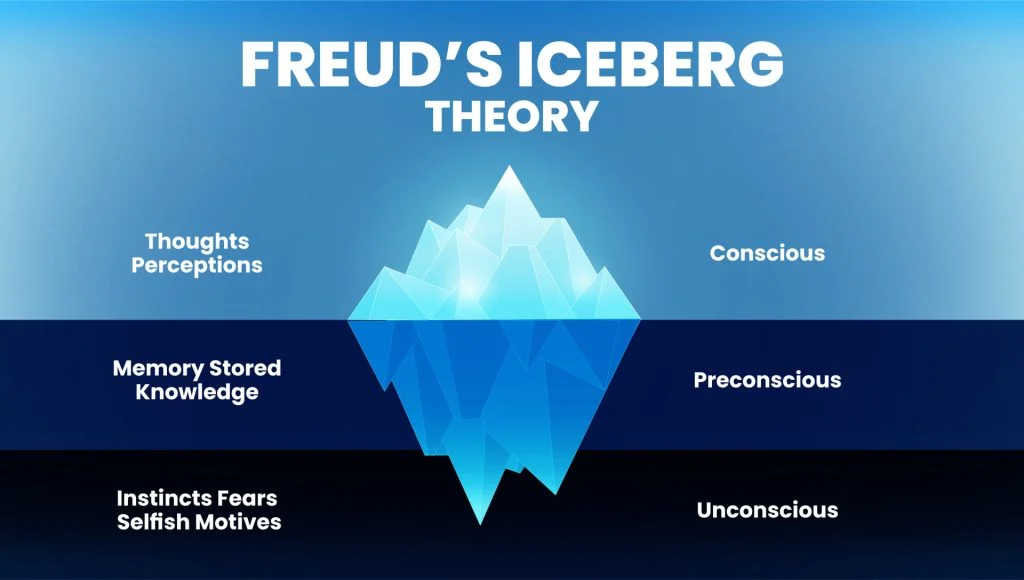
\includegraphics[width=\columnwidth, keepaspectratio]{FreudIcebergTheory}
	\caption{Sigmund Freud's Iceberg Theory}
	\label{Fig:fig1}
\end{figure}

The third type of category of mind is the most mysterious and powerful which is the unconscious mind. It operates beyond our conscious awareness. It is the part of our mind which contains thoughts, memories and emotions that we are not aware of, but that still influence our behaviour and feelings drastically. Conscious mind contains short-term memory. The content stored inside this type of mind can be changed easily on the other hand, the subconscious mind has long-term memory. It can store thoughts longer than the conscious mind which are difficult to change and involves practising something continuously, developing habits by doing continuous efforts in order to change the mindset. The unconscious mind has permanent memory which is almost impossible to be changed by any type of effort. It is the primary source of the human behaviour and personality. It is just like the default personality of a person. These three levels of mind can be understood by the Sigmund Freud's Iceberg Theory as shown in the figure\ref{Fig:fig1}.